A continuación se presentan consultas adicionales para cumplir con los requerimientos del trabajo práctico, junto con las consideraciones tomadas para su resolución y los resultados obtenidos. El código fuente y los resultados completos pueden encontrarse en el notebook \href{https://github.com/patricioibar/datos-tp1/blob/main/consultas_propias.ipynb}{\texttt{consultas\_propias.ipynb}}.

Las siguientes consultas fueron realizadas intentando cubrir las visualizaciones que se piden en la propuesta del trabajo práctico. Estas requieren la comparación de los siguientes tipos de variables:
\begin{enumerate}
    \item Una continua con una línea de tiempo.
    \item Una discreta con una continua.
    \item Una discreta con una discreta.
    \item Una continua con otra continua.
\vspace{-1em}
\end{enumerate}
Además, se agregaron las siguientes visualizaciones adicionales:
\vspace{-1em}
\begin{enumerate}
    \setcounter{enumi}{4}
    \item Un heatmap.
    \item Línea de regresión.
    \item Boxplot.
    \item Treemap.
\end{enumerate}

\subsubsection{Evolución del ingreso neto de dólares a lo largo del tiempo}

Para calcular el ingreso neto de dólares, utilicé la tabla \texttt{orders} que contiene el tipo de cambio utilizado en cada orden.\\
Consideré el ingreso neto como la diferencia entre el total pagado por orden y el total de descuentos e impuestos aplicados. La fórmula que surge es la siguiente:
\[\texttt{Ingreso Neto} = \texttt{Total Pagado} - \texttt{Descuentos} - \texttt{Impuestos}\]

Para conseguir una evolución a lo largo del tiempo y poder graficarlo como una variable continua, agrupé los datos por fecha de creación de la orden, sumando las columnas de ingreso neto.

\begin{lstlisting}[language=Python, xleftmargin=25pt, xrightmargin=25pt]
data = orders.loc[orders.currency == "USD"][["date","total_amount","discount_amount","tax_amount"]]
data["net_income"] = data["total_amount"] - data["discount_amount"] - data["tax_amount"]
data = data.groupby("date")["net_income"].sum().reset_index()
\end{lstlisting}

\begin{figure}[H]
    \centering
    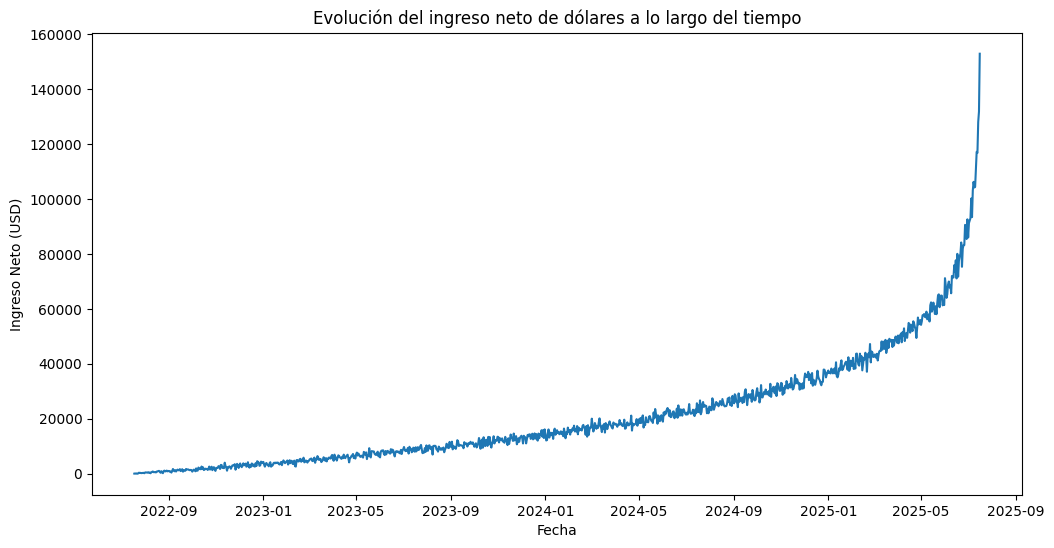
\includegraphics[width=0.8\textwidth]{imagenes/consultas_propias/evolucion_ingreso_neto.png}
    \caption{Evolución del ingreso neto de dólares a lo largo del tiempo.}
    \label{fig:ingreso_neto}
\end{figure}

Puede observarse en la figura \ref{fig:ingreso_neto} que el ingreso neto de dólares ha tenido una tendencia creciente muy marcada a lo largo del tiempo, similar a la encontrada en la figura \ref{fig:cantidad_de_ordenes_por_fecha}. Esto nos da la idea que el ingreso neto aumenta a medida que aumenta la cantidad de órdenes.

\subsubsection{Cantidad de dólares gastados por método de pago por clientes militares activos}

Se considera que un cliente es `militar' si su dirección tiene el estado `AA', `AE' o `AP'. Además, se considera que un cliente es `activo' si la columna \texttt{is\_active} de la tabla \texttt{customers} es verdadera.

Primero filtré los clientes que tienen direcciones militares y que tienen la columna \texttt{is\_active} en verdadero, y conservé únicamente los IDs de los clientes. Luego, filtré la tabla \texttt{orders} para quedarme con las órdenes realizadas por estos clientes y que estén en dólares, utilizando un llamado a \texttt{loc} y otro a \texttt{merge}. Finalmente, agrupé por método de pago y sumé el total gastado.

\begin{lstlisting}[language=Python, xleftmargin=25pt, xrightmargin=25pt]
military_states = ['AA', 'AE', 'AP']
active_military_customers = customers
        .loc[(customers['is_active']) & (customers['state'].isin(military_states))]['customer_id']
        .reset_index()

active_military_orders = orders
        .loc[orders.currency == "USD"]
        .merge(active_military_customers, on='customer_id', how='inner')
        
payment_method_sum = active_military_orders.groupby('payment_method')['total_amount'].sum()
\end{lstlisting}

\begin{figure}[H]
    \centering
    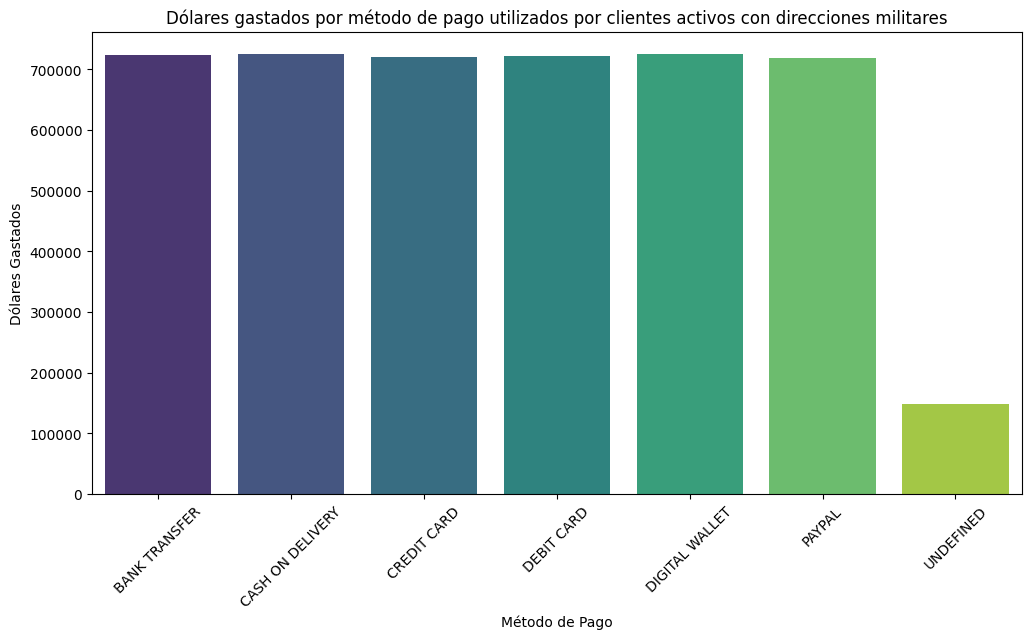
\includegraphics[width=0.8\textwidth]{imagenes/consultas_propias/dolares_militares.png}
    \caption{Cantidad de dólares gastados por método de pago por clientes activos con direcciones militares.}
    \label{fig:dolares_militares}
\end{figure}

Podemos observar una cantidad similar de dólares gastados en cada método de pago, solamente notando una diferencia notable en el método de pago `undefined', que tiene un gasto considerablemente menor.

\subsubsection{Distribución de calificaciones según segmento de cliente.}

Para esta consulta combiné las tablas \texttt{customers} y \texttt{reviews} utilizando un llamado a \texttt{merge}, ya que necesitaba la columna \texttt{customer\_segment} de la tabla \texttt{customers} y la columna \texttt{rating} de la tabla \texttt{reviews}. \\
Luego, para calcular la distribución de calificaciones debería contar las apariciones de cada calificación (de 1 a 5) por cada segmento de cliente y luego dividir por el total de reviews en ese segmento. Encontré que esto puede hacerse utilizando únicamente el método \texttt{value\_counts} estableciendo como verdadero el parámetro \texttt{normalize}.
\begin{lstlisting}[language=Python, xleftmargin=20pt, xrightmargin=20pt]
reviews = reviews.merge(customers[['customer_id', 'customer_segment']], on='customer_id', how='left')
reviews.fillna({'customer_segment': 'UNDEFINED'}, inplace=True)
data = reviews.groupby('customer_segment')['rating'].value_counts(normalize=True).unstack()
\end{lstlisting}
Decidí completar los valores faltantes en la columna \texttt{customer\_segment} con el valor `UNDEFINED', ya que no se puede inferir de ninguna manera el valor para esa columna, pero aún quería conservar todas las reviews en el análisis. 

\begin{figure}[H]
    \centering
    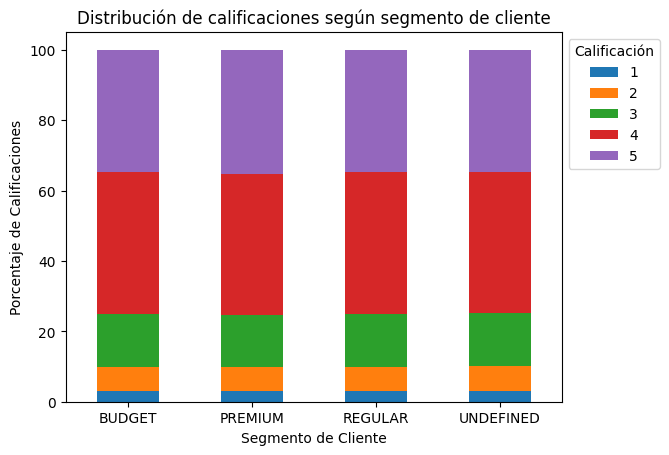
\includegraphics[width=0.8\textwidth]{imagenes/consultas_propias/calificaciones_segmentos.png}
    \caption{Distribución de calificaciones según segmento de cliente.}
    \label{fig:distribucion_calificaciones}
\end{figure}

Pueden observarse nuevamente distribuciones muy uniformes, sin una diferencia notable entre los segmentos de clientes. Puede identificarse que la mayoría de calificaciones son de 4 y 5 estrellas, y que las calificaciones de 1 estrella son las menos frecuentes.

\subsubsection{Relación entre stock disponible y ventas de unidades de zapatos}

Realicé esta consulta con la idea de poder ver si existe alguna relación entre la cantidad de stock disponible y la cantidad de unidades vendidas de zapatos. Quería ver si a mayor stock disponible, mayor cantidad de ventas, o si por el contrario no existe una relación entre estas variables.

Para esto, consideré que el stock encontrado en la tabla de \texttt{products} es el stock actual del producto. Se compara contra las ventas históricas de unidades de ese producto, que se encuentran en la tabla \texttt{order\_items}. No fue posible filtrar según tiempos de ventas, ya que esa información no se encuentra en la tabla \texttt{order\_items}, y no es posible cruzar esta tabla con la tabla \texttt{orders} ya que no identificadores de órdenes en común.

Para realizar esta consulta primero identifiqué los IDs de las categoráis de zapatos, y los utilicé para buscar los IDs de los productos que pertenecen a estas categorías. Luego, utilicé estos IDs para filtrar la tabla \texttt{order\_items} y quedarme con las ventas de unidades de zapatos. Agrupé por ID de producto y sumé la cantidad de unidades vendidas. Finalmente, realicé un \texttt{merge} con la tabla \texttt{products} para obtener el stock disponible de cada producto, y con la previemante generada \texttt{shoes\_categories} para obtener los nombres de las categorías.

\begin{figure}
\begin{lstlisting}[language=Python, xleftmargin=10pt, xrightmargin=10pt]
shoes_categories = categories[categories['parent_category'] == 'SHOES'][['category_id', 'category_name']]
shoes_products = products[products['category_id'].isin(shoes_categories['category_id'])]

shoes_order_items = items[items['product_id'].isin(shoes_products['product_id'])]
.groupby('product_id')['quantity'].sum().reset_index()

data = shoes_order_items.merge(
products[['product_id', 'stock_quantity', 'category_id']], on='product_id', how='left'
)
data = data.merge(
shoes_categories[['category_id', 'category_name']], on='category_id', how='left'
)
\end{lstlisting}
\end{figure}

Me pareció curioso que al graficar esto en un scatter plot, la leyenda de colores no contenía únicamente las categorías de zapatos, sino que también aparecían categorías de otros tipos de productos. Esto se debía a que la columna \texttt{category\_name} es de tipo \texttt{category} y aún luego de ser filtrada y mergeada, conservaba los valores originales. Para solucionar esto, convertí la columna a tipo \texttt{string}.

\begin{figure}[H]
    \centering
    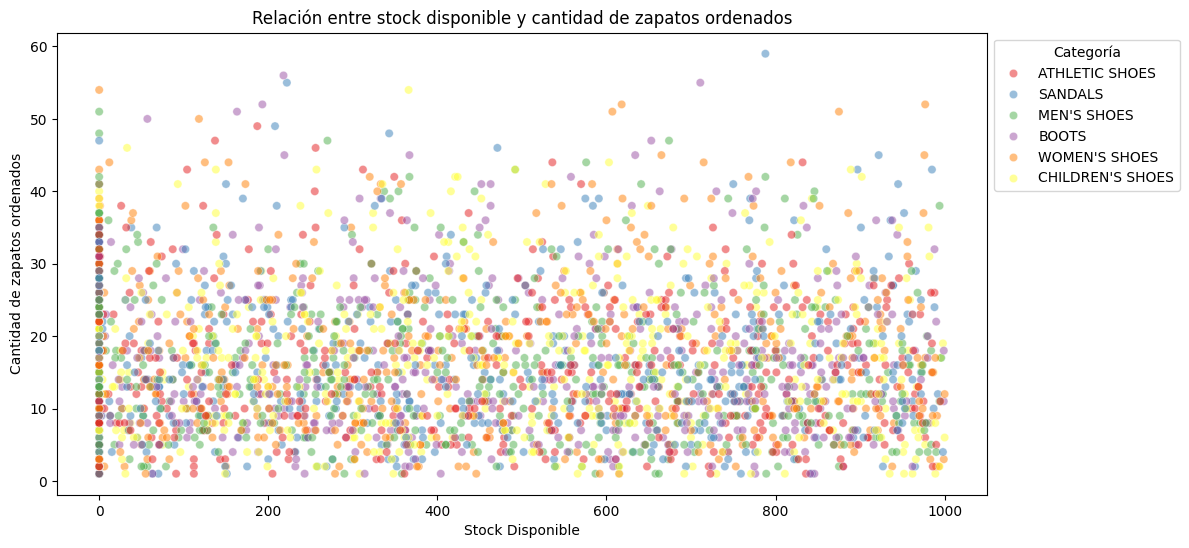
\includegraphics[width=0.8\textwidth]{imagenes/consultas_propias/stock_zapatos.png}
    \caption{Relación entre stock disponible y ventas de unidades de zapatos.}
    \label{fig:stock_vs_ventas}
\end{figure}

Lamentablemente, no se observa una relación clara entre las variables. Tampoco se puede observar una diferencia clara entre el comportamiento de las distintas categorías de zapatos.\\
Puede observarse una concentración elevada en los puntos en el valor de x=0, que indica que hay muchos productos de zapatos que no tienen stock.

\subsubsection{Rating promedio por categoría padre y segmento de cliente}

Para esta consulta combiné las tablas \texttt{reviews}, \texttt{products}, \texttt{categories} utilizando llamados a \texttt{merge}, ya que necesitaba la columna \texttt{rating} de la tabla \texttt{reviews}, la columna \texttt{category\_id} de la tabla \texttt{products}, la columna \texttt{parent\_category} de la tabla \texttt{categories}. También necesitaba la columna \texttt{customer\_segment} de la tabla \texttt{customers}, que ya se encontraba en la tabla \texttt{reviews} una consulta anterior.\\
Luego agrupé por categoría padre y segmento de cliente, y calculé el promedio de las calificaciones.
\begin{lstlisting}[language=Python, xleftmargin=20pt, xrightmargin=20pt]
reviews = reviews.merge(products[['product_id', 'category_id']], on='product_id', how='left')
reviews = reviews.merge(categories[['category_id', 'parent_category']], on='category_id', how='left')
data = reviews.groupby(['parent_category', 'customer_segment'])['rating'].mean().unstack()
\end{lstlisting}

\begin{figure}[H]
    \centering
    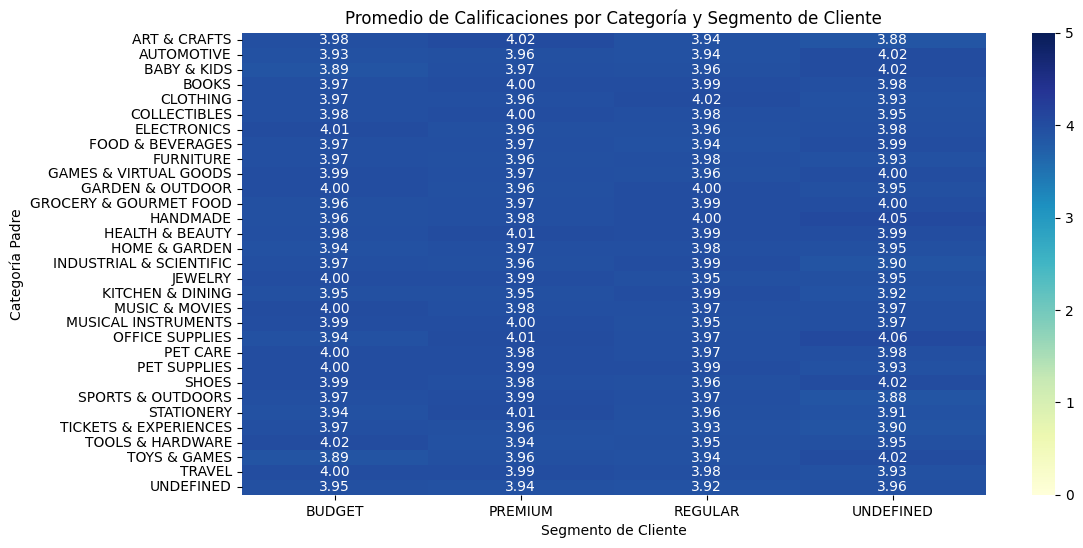
\includegraphics[width=0.8\textwidth]{imagenes/consultas_propias/rating_promedio_padre.png}
    \caption{Rating promedio por categoría padre y segmento de cliente.}
    \label{fig:rating_promedio}
\end{figure}
\vspace{-1em}
\begin{figure}[H]
    \centering
    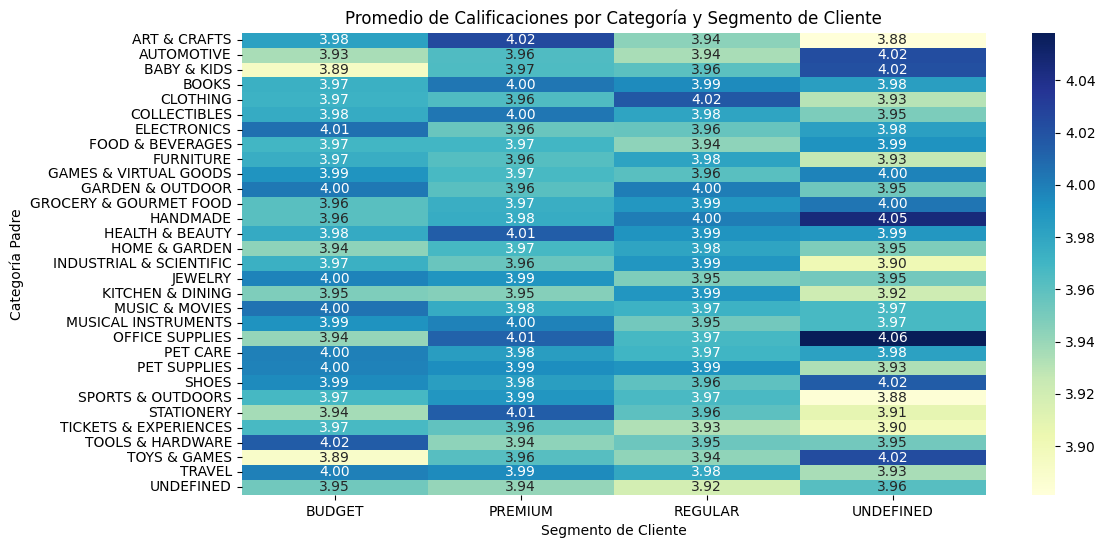
\includegraphics[width=0.8\textwidth]{imagenes/consultas_propias/rating_promedio_padre_closer.png}
    \caption{Rating promedio por categoría padre y segmento de cliente, con una escala de color más cercana.}
    \label{fig:rating_promedio_closer}
\end{figure}
Puede observarse en la figura \ref{fig:rating_promedio} que todos los ratings promedio se encuentran muy cercanos a 4, obteniendo un heatmap de color casi uniforme. \\
En la figura \ref{fig:rating_promedio_closer} se ajusta la escala de colores para poder observar mejor las diferencias entre los ratings promedio. La escala va aproximadamente desde 3.85 hasta 4.10, lo cual es bastante pequeño. Aún con esta escala ajustada, se pueden observar que la mayoría de ratings se encuentran muy cercanos entre sí.

\subsubsection{Relación entre precio de Smartphones activos y sus unidades vendidas}

Originalmente, esta consulta se había planteado como la relación entre el precio de smartphones activos y su rating promedio. Sin embargo, como se observó en consultas anteriores, los ratings promedio de los productos se encuentran todos muy cercanos entre sí, por lo que no sería posible observar una relación clara entre estas variables. Por este motivo, se decidió cambiar la variable a comparar contra el precio por la cantidad de unidades vendidas.

Para realizar esta consulta, primero identifiqué el ID de la categoría `SMARTPHONES', y lo utilicé para buscar los IDs de los productos que pertenecen a esta categoría y que además están activos. Luego, utilicé estos IDs para filtrar la tabla \texttt{order\_items} y agrupé por ID de producto para sumar la cantidad de unidades vendidas. Finalmente, realicé un \texttt{merge} con la tabla \texttt{products} para obtener el precio de cada producto.

\begin{lstlisting}[language=Python, xleftmargin=40pt, xrightmargin=40pt]
smartphone_category_id = categories[
    categories['category_name'] == 'SMARTPHONES'
    ]['category_id'].iloc[0]

active_smartphones = products[
    (products['category_id'] == smartphone_category_id) & (products['is_active'])
    ][['product_id', 'price']]

data = items[items['product_id'].isin(active_smartphones['product_id'])]
            .groupby('product_id')['quantity'].sum().reset_index()

data = data.merge(active_smartphones[['product_id', 'price']], on='product_id', how='left')
\end{lstlisting}

\begin{figure}[H]
    \centering
    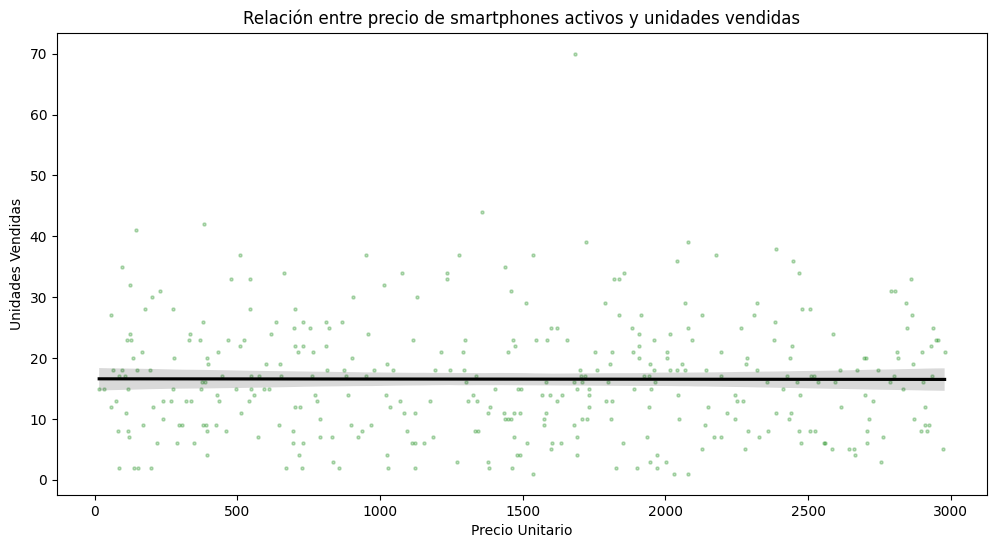
\includegraphics[width=0.8\textwidth]{imagenes/consultas_propias/smartphones.png}
    \caption{Relación entre precio de smartphones activos y unidades vendidas.}
    \label{fig:smartphone_price_vs_quantity}
\end{figure}

Una vez más, la distribución de los puntos es bastante uniforme, sin una relación clara entre las variables. No se observa que a mayor precio, mayor o menor cantidad de unidades vendidas. Más aún, puede observarse que la línea de regresión es prácticamente horizontal, indicando que no existe una relación lineal entre las variables sino que se distribuyen de manera uniforme.

\subsubsection{Distribución del descuento unitario para las 5 categorías de producto más vendidas}

Para hallar el descuento unitario de la venta de un producto, supuse que la columna \texttt{discount\_amount} de la tabla \texttt{order\_items} representa el descuento total aplicado a la venta de ese producto en esa orden. Por lo tanto, el descuento unitario puede hallarse dividiendo este valor por la cantidad de unidades vendidas de ese producto en esa orden.

Primero encontré las 5 categorías de productos más vendidas sumando la cantidad de unidades vendidas por categoría. Para esto, realicé un \texttt{merge} entre las tablas \texttt{order\_items} y \texttt{products} para poder obtener el ID de la categoría de cada producto vendido. Aproveché este  paso para quedarme únicamente con las columnas que voy a utilizar en esta consulta. Luego, agrupé por ID de categoría y sumé la cantidad de unidades vendidas, quedándome con las 5 categorías con mayor cantidad de ventas utilizando \texttt{nlargest}. \\
Luego, filtré las filas de la tabla \texttt{order\_items} para quedarme únicamente con los productos que pertenecen a estas categorías, para poder visuaizar la distribución de esos valores. Finalmente, calculé el descuento unitario y graficé su distribución utilizando violinplot.

\begin{lstlisting}[language=Python, xleftmargin=19pt, xrightmargin=19pt]
items_categories = items.merge(
    products[['product_id', 'category_id']], on='product_id', how='left'
    )[['product_id', 'category_id', 'quantity', 'discount_amount']]

top_5_categories = items_categories.groupby('category_id')['quantity'].sum().nlargest(5)

items_categories = items_categories[items_categories['category_id'].isin(top_5_categories.index)]
items_categories['unit_discount'] = items_categories['discount_amount'] / items_categories['quantity']
\end{lstlisting}

Para quedarme con los nombres de las categorías en lugar de sus IDs, armé un diccionario a partir de la tabla \texttt{categories} y utilicé el método \texttt{map} para crear una nueva columna con los nombres.

\begin{lstlisting}[language=Python, xleftmargin=35pt, xrightmargin=35pt]
categories_names = categories[['category_id', 'category_name']]
    .loc[categories['category_id'].isin(top_5_categories.index)].reset_index()

    category_name_map = {}
for _, row in categories_names.iterrows():
    category_name_map[row['category_id']] = row['category_name']

items_categories['category_id'] = items_categories['category_id'].map(category_name_map)
items_categories.rename(columns={'category_id': 'category_name'}, inplace=True)
\end{lstlisting}

También reemplacé los valores nulos de la columna \texttt{unit\_discount} por 0, ya que supuse que estos valores se producen cuando no hubo descuento aplicado en la venta del producto.

\begin{figure}[H]
    \centering
    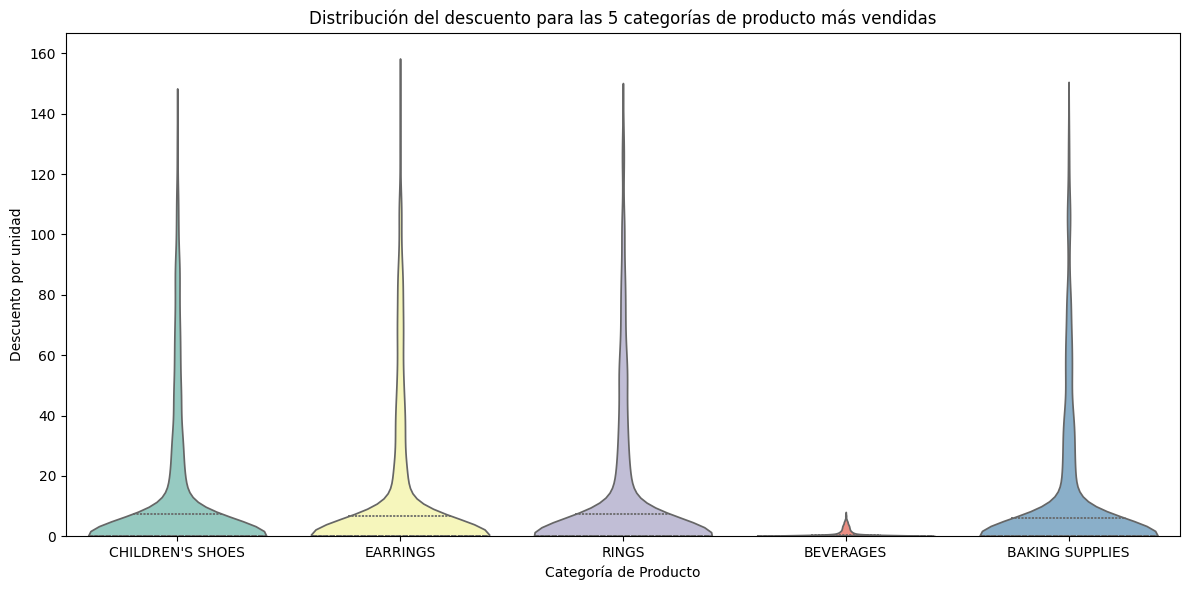
\includegraphics[width=0.8\textwidth]{imagenes/consultas_propias/descuento_categorias.png}
    \caption{Distribución del descuento unitario para las 5 categorías de producto más vendidas.}
    \label{fig:descuento_categorias}
\end{figure}

Mostré los violin plots `truncados' en la parte inferior ya que el descuento unitario no puede ser negativo. \\
Notar cómo la distribución de las categorías es casi idéntica, aún para categorías de productos diferentes como `CHILDREN'S SHOES', `RINGS', y `BAKING SUPPLIES'. La única excepción es la categoría `BEVERAGES', que tiene una distribución un poco más concentrada en valores bajos de descuento unitario.

\subsubsection{Unidades de productos robados por categoría y subcategoría de producto}

Para esta consulta, consideré que un producto fue robado si la columna razón del registro de la tabla \texttt{inventory\_logs} es igual a `STOLEN', y el valor de la columna \texttt{quantity\_change} es menor a 0, lo cual indicaría que el producto fue sustraído del inventario.

Primero filtré la tabla \texttt{inventory\_logs} para quedarme únicamente con los registros que cumplen estas condiciones. Luego, mergeé con la tabla \texttt{products} para obtener el ID de la categoría de cada producto robado, y con la tabla \texttt{categories} para obtener los nombres de las categorías y subcategorías. Finalmente, agrupé por categoría y subcategoría, sumando la cantidad de unidades robadas.\\
Finalmenente, tuve que quedarme con los valores absolutos de la cantidad de unidades robadas, ya que al ser valores negativos no se podían graficar en un treemap.

\begin{lstlisting}[language=Python, xleftmargin=55pt, xrightmargin=55pt]
stealed_orders = inventory[
    (inventory['reason'] == 'THEFT') & (inventory['quantity_change'] < 0)
    ][['quantity_change', 'product_id']]

stealed_orders = stealed_orders.merge(
    products[['product_id', 'category_id']], on='product_id'
    )
stealed_orders = stealed_orders.merge(
    categories[['category_id', 'category_name', 'parent_category']], on='category_id'
    )[['quantity_change', 'category_name', 'parent_category']]

stealed_orders = stealed_orders.groupby(
    ['parent_category', 'category_name']
)['quantity_change'].sum().reset_index()

stealed_orders['quantity_change'] = stealed_orders['quantity_change'].abs()
\end{lstlisting}

Pueden observarse en la figura \ref{fig:robos_treemap} cantidades similares para todas las categorías padre y subcategorías, sin una diferencia notable entre ellas. Esto en un escenario real resultaría extraño, ya que se esperaría que algunas categorías de productos sean más propensos a ser robadas que otros.\\
La gran cantidad de categorías y subcategorías dificulta la visualización, pero puede observarse que todas tienen valores similares. \\
En el \href{https://github.com/patricioibar/datos-tp1/blob/main/consultas_propias.ipynb}{notebook} puede encontrarse el código para graficar el treemap de la figura \ref{fig:robos_treemap} utilizando la librería \texttt{plotly}, el cual genera una versión interactiva del gráfico en la que se pueden visualizar mejor las categorías de manera individual.

Adicionalmente, agregué un gráfico de tipo sunburst, que es similar al treemap pero muestra la jerarquía de categorías de manera radial. El código para generarlo y poder visuaizarlo de forma interactiva también puede encontrarse en el \href{https://github.com/patricioibar/datos-tp1/blob/main/consultas_propias.ipynb}{notebook} \\
En este gráfico puede observarse de manera más clara que todas las categorías y categorías padre tienen valores similares.

\begin{figure}[H]
    \centering
    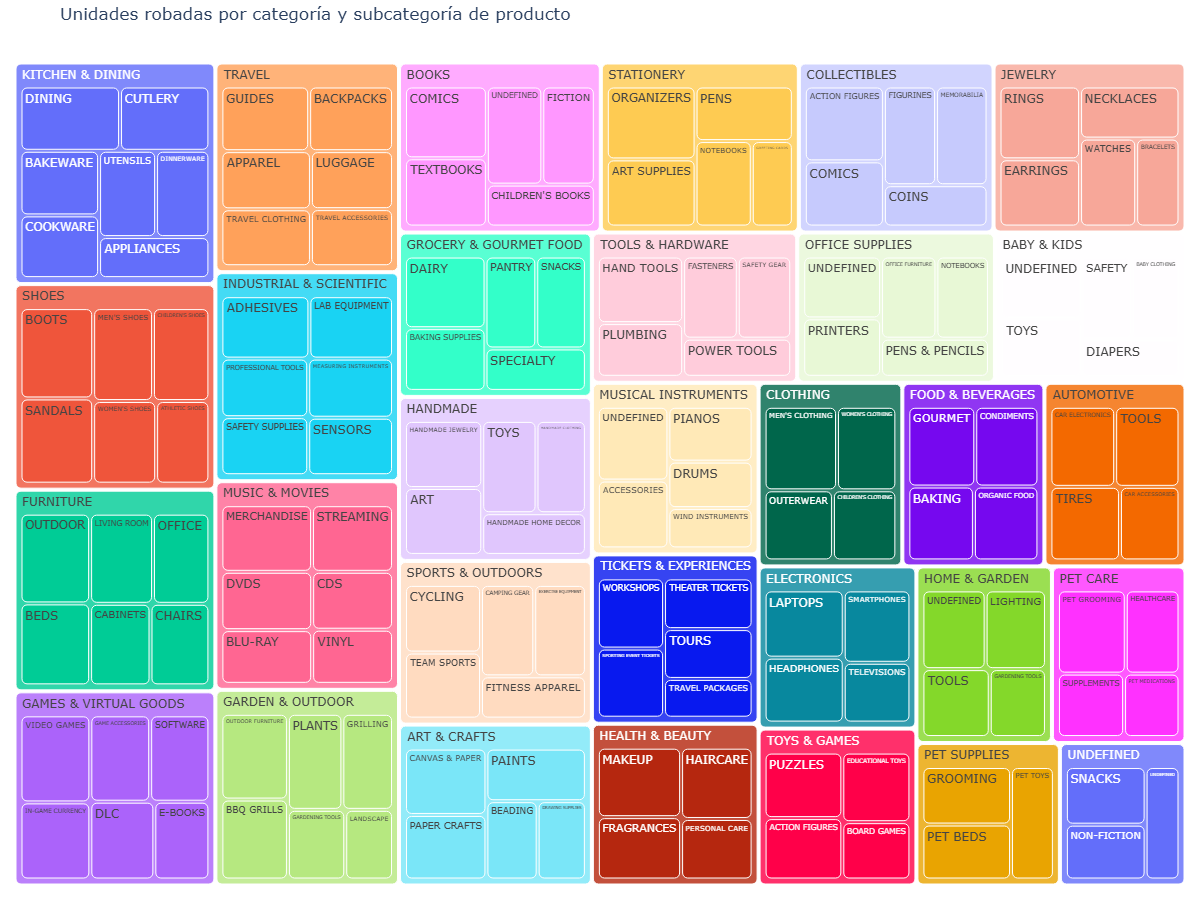
\includegraphics[width=0.8\textwidth]{imagenes/consultas_propias/treemap.png}
    \caption{Unidades de productos robados por categoría y subcategoría de producto.}
    \label{fig:robos_treemap}
\end{figure}

\begin{figure}[H]
    \centering
    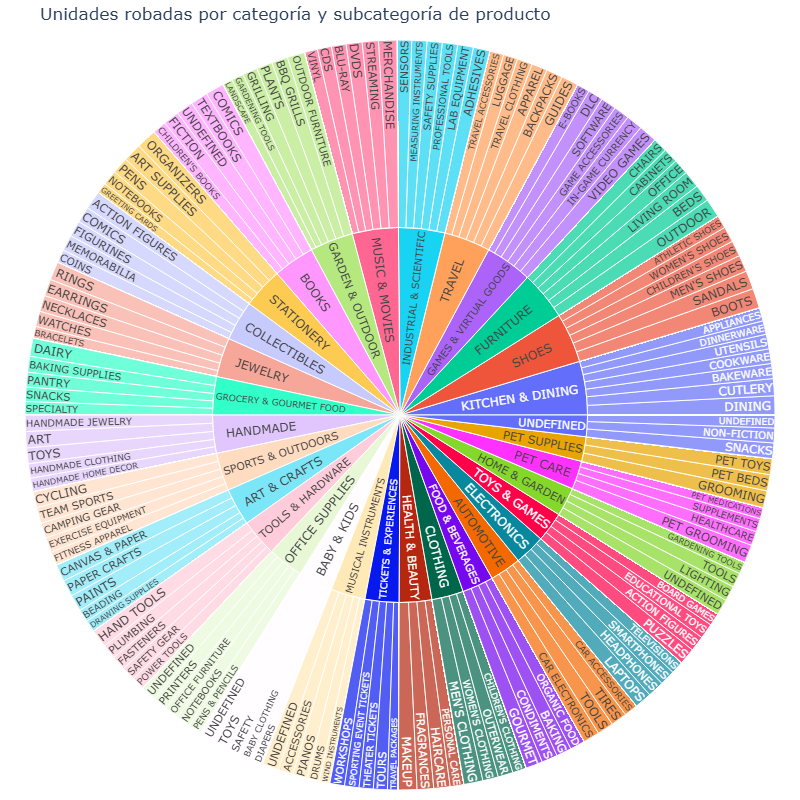
\includegraphics[width=0.6\textwidth]{imagenes/consultas_propias/sunburst.png}
    \caption{Unidades de productos robados por categoría y subcategoría de producto, visualizado como sunburst.}
    \label{fig:robos_sunburst}
\end{figure}
